\documentclass[aspectratio=169,11pt]{beamer}

\usepackage{graphicx}
\usepackage{booktabs}
\usepackage{array}
\usepackage{amsmath}
\usepackage{tikz}
\usetikzlibrary{shapes.geometric, arrows.meta, positioning}

% ---- clean light-grey minimalist theme ----
\usetheme{default}
\usefonttheme{serif}
\setbeamertemplate{navigation symbols}{}
\definecolor{bggray}{RGB}{237,237,237}
\definecolor{accent}{RGB}{40,72,120}
\setbeamercolor{background canvas}{bg=bggray}
\setbeamercolor{frametitle}{fg=black,bg=bggray}
\setbeamercolor{itemize item}{fg=accent}
\setbeamerfont{frametitle}{size=\LARGE,series=\mdseries}
\setbeamertemplate{frametitle}[default][center]
\setbeamertemplate{itemize item}{\textbullet}
\renewcommand{\arraystretch}{1.25}

% ---- BMSCE logo, top-right of every titled slide ----
\addtobeamertemplate{frametitle}{}{%
\begin{tikzpicture}[remember picture,overlay]
\node[anchor=north east,yshift=-1pt,xshift=-3pt] at (current page.north east)
  {
\includegraphics[height=0.95cm]{figs/bmsce_logo.png}};
\end{tikzpicture}}

\begin{document}

% ============ TITLE ============
\begin{frame}[plain]
\begin{tikzpicture}[remember picture,overlay]
\node[anchor=north east,yshift=-6pt,xshift=-8pt] at (current page.north east)
  {
\includegraphics[height=1.5cm]{figs/bmsce_logo.png}};
\end{tikzpicture}
\vspace{0.4cm}
\begin{center}
{\LARGE\bfseries RF-Based Drone Identification\\[2pt]
Using Machine Learning}\\[6pt]
{\footnotesize\color{gray}[23ET7PE3ML]}\\[6pt]
{\normalsize Department of Electronics and Telecommunication Engineering}\\[4pt]
{\footnotesize BMS College of Engineering, Bengaluru}
\end{center}
\vspace{0.6cm}
\begin{columns}[t]
\begin{column}{0.45\textwidth}
{\large Guided by}\\[3pt]
Dr. C Gururaj\\
Professor, Department of Electronics and Communication
\end{column}
\begin{column}{0.5\textwidth}
{\large Presented by}\\[3pt]
\begin{tabular}{@{}ll@{}}
Utkarsh Sinha & (1BM23ET055)\\
Vishal Joshy & (1BM23ET058)\\
Yash Gupta & (1BM23ET061)\\
\end{tabular}
\end{column}
\end{columns}
\end{frame}

% ============ INTRODUCTION + PROBLEM ============
\begin{frame}{Introduction and Problem Definition}
\begin{itemize}
\item Unmanned Aerial Vehicles (UAVs) transmit continuous \textbf{Radio
Frequency (RF)} control signals to their operators, enabling \textbf{passive
detection} without line of sight, unlike optical or radar sensing.
\item These links operate in the \textbf{2.4~GHz ISM band} (Industrial,
Scientific and Medical). This band is chosen because it is licence-free
worldwide and balances range against antenna size; lower bands sacrifice data
rate, higher bands sacrifice range and obstacle penetration.
\item Detecting \textbf{presence} alone is insufficient; a practical system must
also determine the \textbf{drone family} and its \textbf{operating condition}
to assess threat level.
\item The 2.4~GHz band is shared with \textbf{Wi-Fi and Bluetooth}, so recorded
signals are noisy and classification is non-trivial.
\item Segments extracted from a single recording are highly correlated;
assigning them to both training and test sets causes \textbf{data leakage} and
inflates measured accuracy.
\item \textbf{Objective:} classify drone presence, family and operating
condition from the \textbf{DroneRF} dataset under a \textbf{leakage-aware}
evaluation.
\end{itemize}
\end{frame}

% ============ METHODOLOGY (EQUAL BLOCKS) ============
\begin{frame}{Proposed Methodology}
\centering
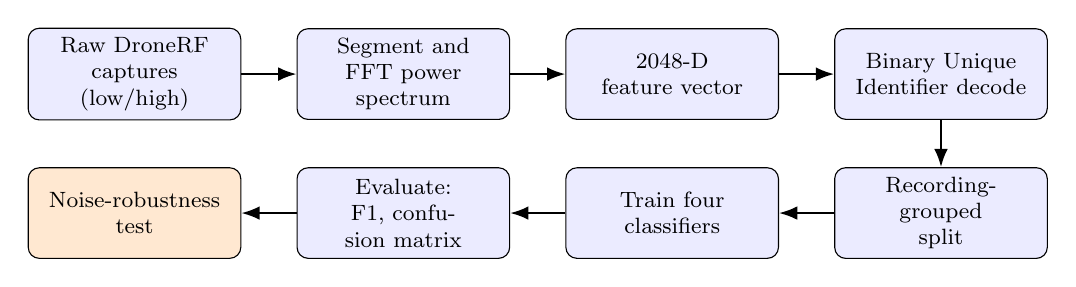
\begin{tikzpicture}[
  node distance=0.6cm and 0.7cm,
  box/.style={rectangle, draw, rounded corners, align=center,
    font=\footnotesize, minimum width=2.7cm, minimum height=1.15cm,
    text width=2.4cm, fill=blue!8},
  save/.style={rectangle, draw, rounded corners, align=center,
    font=\footnotesize, minimum width=2.7cm, minimum height=1.15cm,
    text width=2.4cm, fill=orange!18},
  arr/.style={-{Latex}, thick}
]
\node[box] (raw) {Raw DroneRF\\captures (low/high)};
\node[box, right=of raw] (seg) {Segment and\\FFT power spectrum};
\node[box, right=of seg] (feat) {2048-D\\feature vector};
\node[box, right=of feat] (label) {Binary Unique\\Identifier decode};
\node[box, below=of label] (split) {Recording-grouped\\split};
\node[box, left=of split] (train) {Train four\\classifiers};
\node[box, left=of train] (eval) {Evaluate:\\F1, confusion matrix};
\node[save, left=of eval] (noise) {Noise-robustness\\test};
\draw[arr] (raw) -- (seg);
\draw[arr] (seg) -- (feat);
\draw[arr] (feat) -- (label);
\draw[arr] (label) -- (split);
\draw[arr] (split) -- (train);
\draw[arr] (train) -- (eval);
\draw[arr] (eval) -- (noise);
\end{tikzpicture}
\vspace{0.3cm}

\footnotesize The \textbf{Fast Fourier Transform (FFT)} converts each time-domain
segment into a frequency fingerprint; three labels are then decoded from a
single filename code.
\end{frame}

% ============ DATASET USED ============
\begin{frame}{Dataset Used: DroneRF}
\footnotesize
\textbf{Why this dataset:} DroneRF is the standard public benchmark for RF-based
drone detection, published with the founding study in this field, which makes
results directly comparable with prior work.
\vspace{0.15cm}

\centering
\scriptsize
\begin{tabular}{|l|c|c|c|}
\hline
\textbf{Class (Family)} & \textbf{BUI codes} & \textbf{Modes} & \textbf{Role} \\
\hline
Background (no drone) & 00000 & 1 & Negative class \\
\hline
Parrot Bebop & 10000--10011 & 4 & Drone family 1 \\
\hline
Parrot AR & 10100--10111 & 4 & Drone family 2 \\
\hline
DJI Phantom & 11000 & 1 & Drone family 3 \\
\hline
\end{tabular}
\vspace{0.2cm}

\raggedright\footnotesize
\textbf{Scale:} approximately \textbf{41~GB} of raw recordings, comprising
\textbf{227 recording pairs}, which yield \textbf{22{,}700} labelled feature
vectors after segmentation.\\
\textbf{BUI} denotes a \textbf{Binary Unique Identifier}, the 5-digit code that
labels every recording (expanded on the next slide).
\end{frame}

% ============ LABEL DECODING + FILE VIEW ============
\begin{frame}{Label Decoding from the Filename}
\begin{columns}[t]
\begin{column}{0.46\textwidth}
\scriptsize
\textbf{Example files on disk:}
\vspace{0.1cm}

\colorbox{black!88}{\color{white}\ttfamily\scriptsize
\begin{minipage}{0.92\linewidth}
\vspace{2pt}
10111H\_3.csv\\
10111L\_3.csv\\[3pt]
\textcolor{green!60}{\# contents (RF samples)}\\
-0.021, 0.034, -0.012,\\
0.045, 0.008, -0.030,\\
0.019, -0.007, 0.041, ...
\vspace{2pt}
\end{minipage}}
\vspace{0.15cm}

\textbf{BUI} = \textbf{Binary Unique Identifier} (5 digits):
the first digit marks drone presence, the next two the drone family, the last
two the operating mode. The letter (H/L) marks the high or low RF sub-band.
\end{column}
\begin{column}{0.5\textwidth}
\scriptsize
\textbf{All three labels decode from the code:}
\vspace{0.15cm}

\begin{tabular}{|l|p{3.0cm}|}
\hline
\textbf{Target} & \textbf{Rule} \\
\hline
Presence (2 classes) & 0 if background, else 1 \\
\hline
Family (4 classes) & background, Bebop, AR or Phantom \\
\hline
Mode (10 classes) & one index per BUI code \\
\hline
\end{tabular}
\vspace{0.2cm}

\footnotesize No manual labelling is required, since the ground truth is
embedded in each filename.
\end{column}
\end{columns}
\end{frame}

% ============ FEATURE EXTRACTION (DETAILED) ============
\begin{frame}{Feature Extraction}
\footnotesize
Raw RF captures are long sequences of amplitude samples that appear as noise in
the time domain. The drone's signature is visible only in the
\textbf{frequency domain}, so the pipeline transforms each segment as follows:
\begin{enumerate}\footnotesize
\item \textbf{Segmentation:} each capture is divided into windows of
$L = 100{,}000$ samples, long enough to hold a stable spectrum yet short enough
to yield many training examples.
\item \textbf{Fast Fourier Transform:} a 2048-point FFT (a power of two, for
computational efficiency) converts each window to the frequency domain; the
upper 1024 bins are retained, as the magnitude spectrum is symmetric.
\[
X_f = \big|\,\mathrm{FFT}_{M}(x - \bar{x})\,\big|,\qquad f = \tfrac{M}{2}+1,\dots,M
\]
\item \textbf{Band fusion:} the low (\texttt{L}) and high (\texttt{H})
sub-bands are concatenated and squared to a \textbf{power spectrum}, giving a
single \textbf{2048-dimensional} vector per segment.
\end{enumerate}
\vspace{0.1cm}
Result: a feature matrix of \textbf{22{,}700~$\times$~2048} for model training.
\end{frame}

% ============ ALGORITHMS ============
\begin{frame}{Classification Models and Rationale}
\scriptsize
\begin{tabular}{|p{2.9cm}|p{4.2cm}|p{4.4cm}|}
\hline
\textbf{Model} & \textbf{Rationale for inclusion} & \textbf{Observed behaviour} \\
\hline
Logistic Regression & Linear baseline; strong performance would imply a
linearly separable task & Perfect on presence and family; weak on mode (0.375) \\
\hline
Random Forest & Bagging ensemble that captures non-linear structure &
Stable; marginally lower on family (0.898) \\
\hline
Support Vector Machine (RBF kernel) & Models curved decision boundaries &
Strong on simple tasks; limited on mode (5000-sample training cap) \\
\hline
XGBoost & Gradient-boosted trees; state of the art on tabular data &
\textbf{Best overall}, and decisively best on the mode task (0.492) \\
\hline
\end{tabular}
\vspace{0.25cm}

\footnotesize All four models perform near-identically on the easy tasks and
separate only on the 10-class operating-mode task, where XGBoost leads. That
task is therefore where the comparison is meaningful.
\end{frame}

% ============ RESULTS ============
\begin{frame}{Classification Results}
\centering
\footnotesize
\begin{tabular}{|l|c|c|c|}
\hline
\textbf{Model} & \textbf{Presence} & \textbf{Family} & \textbf{Mode (5-fold)} \\
\hline
Logistic Regression & 1.000 & 0.999 & 0.375 \\
\hline
Random Forest & 0.978 & 0.898 & 0.378 \\
\hline
Support Vector Machine & 1.000 & 0.977 & 0.160 \\
\hline
XGBoost & \textbf{1.000} & \textbf{1.000} & \textbf{0.492} \\
\hline
\end{tabular}
\vspace{0.3cm}
\begin{itemize}\footnotesize
\item Scores are reported as \textbf{macro-averaged F1}, which is robust to the
class imbalance in the dataset.
\item \textbf{Presence} and \textbf{family} are essentially solved; the 10-class
\textbf{operating-mode} task is hard, with XGBoost leading at 0.492 ($\pm0.009$
over five folds).
\end{itemize}
\end{frame}

% ============ CONFUSION MATRICES ALL MODELS ============
\begin{frame}{Confusion Matrices: All Models (Operating Mode)}
\centering
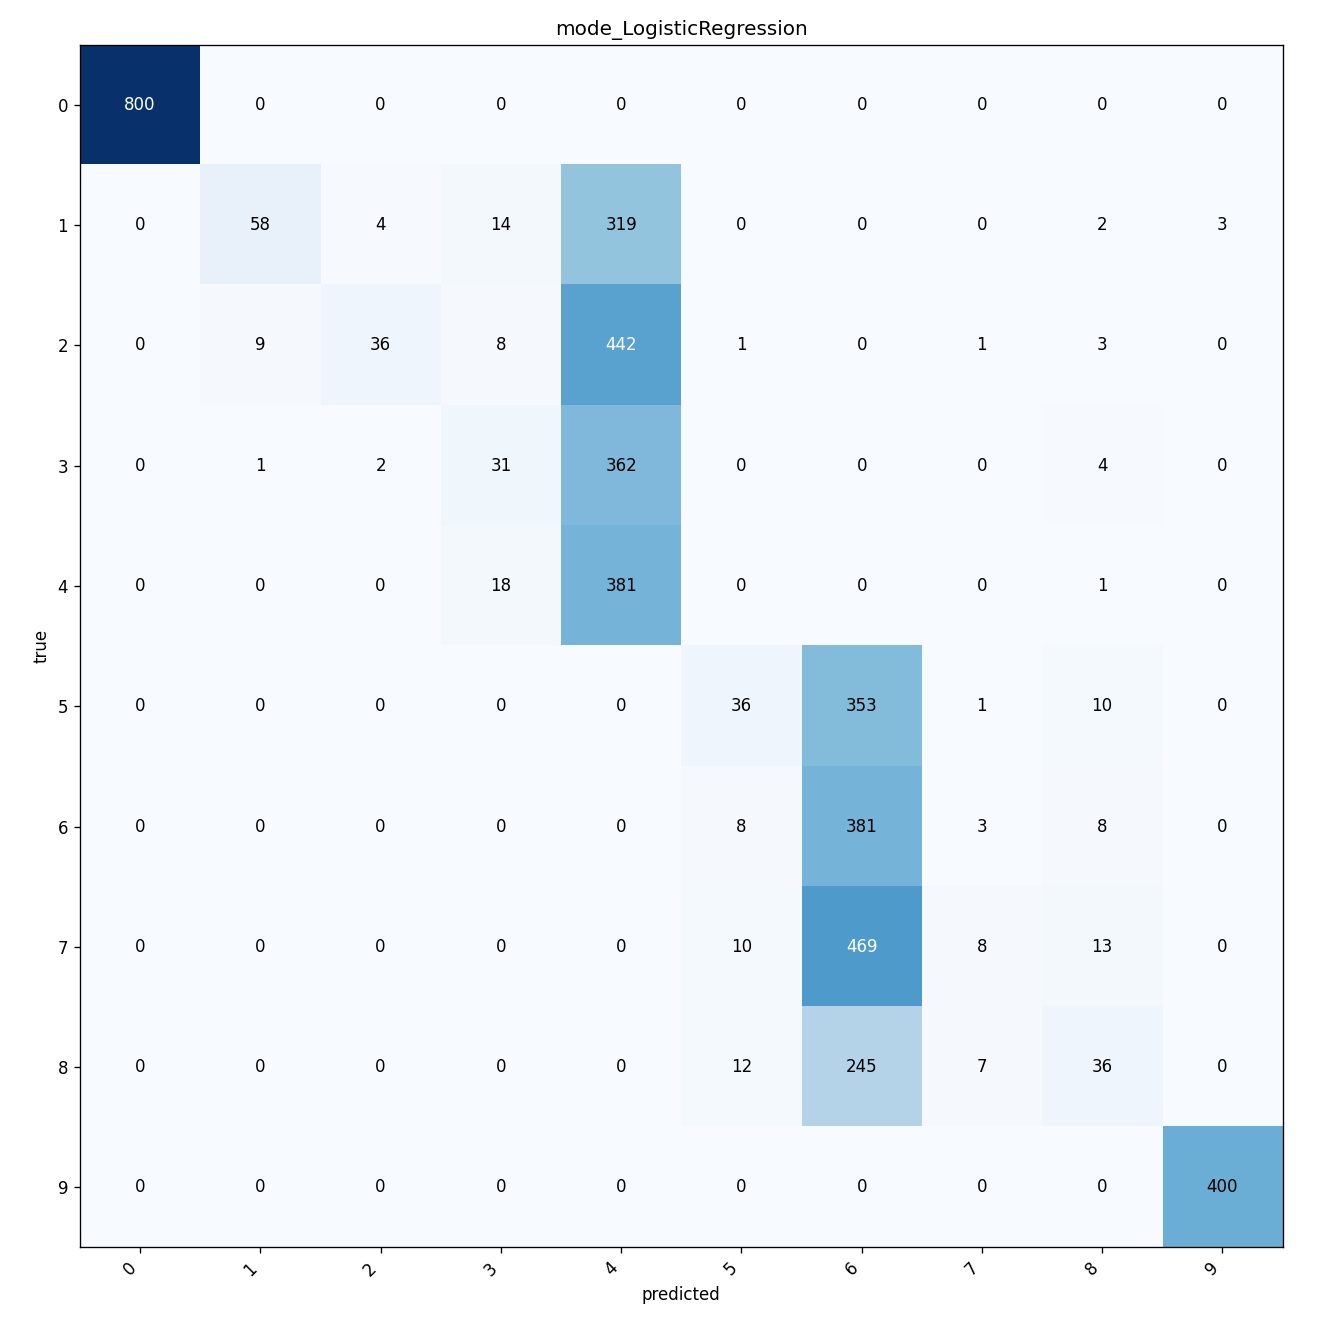
\includegraphics[height=0.40\textheight]{figs/cmmode_LogisticRegression.png}\hfill
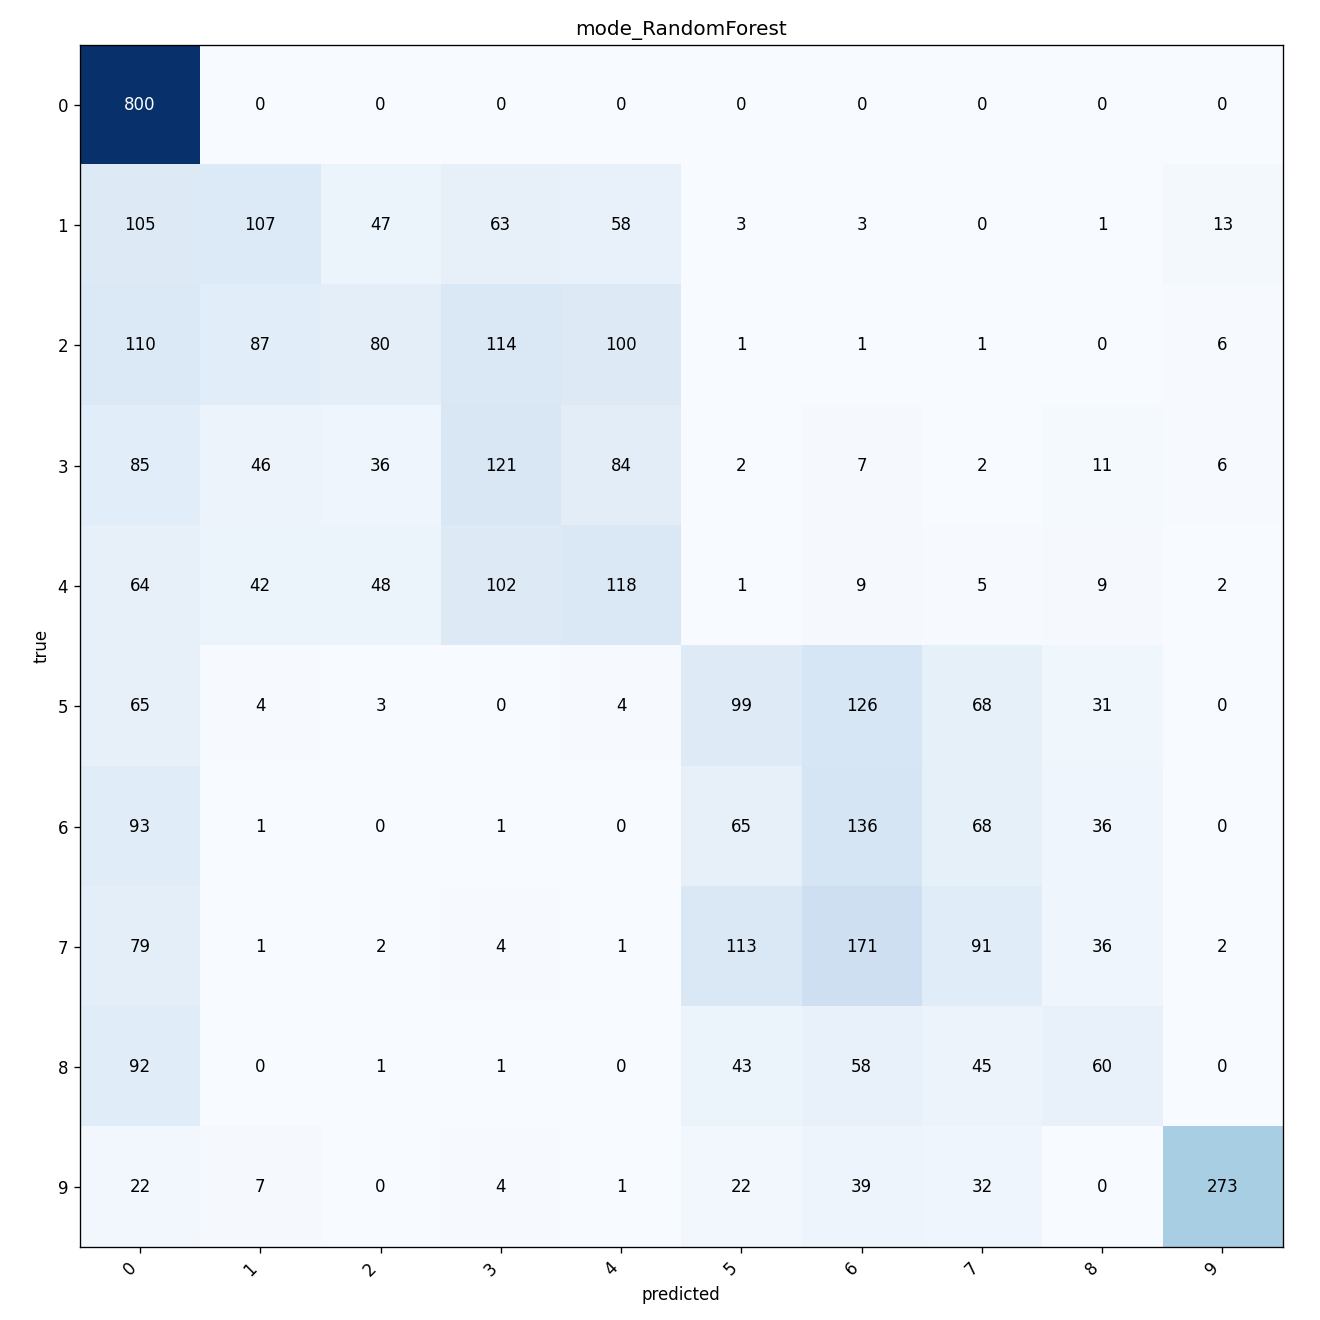
\includegraphics[height=0.40\textheight]{figs/cmmode_RandomForest.png}\\[2pt]
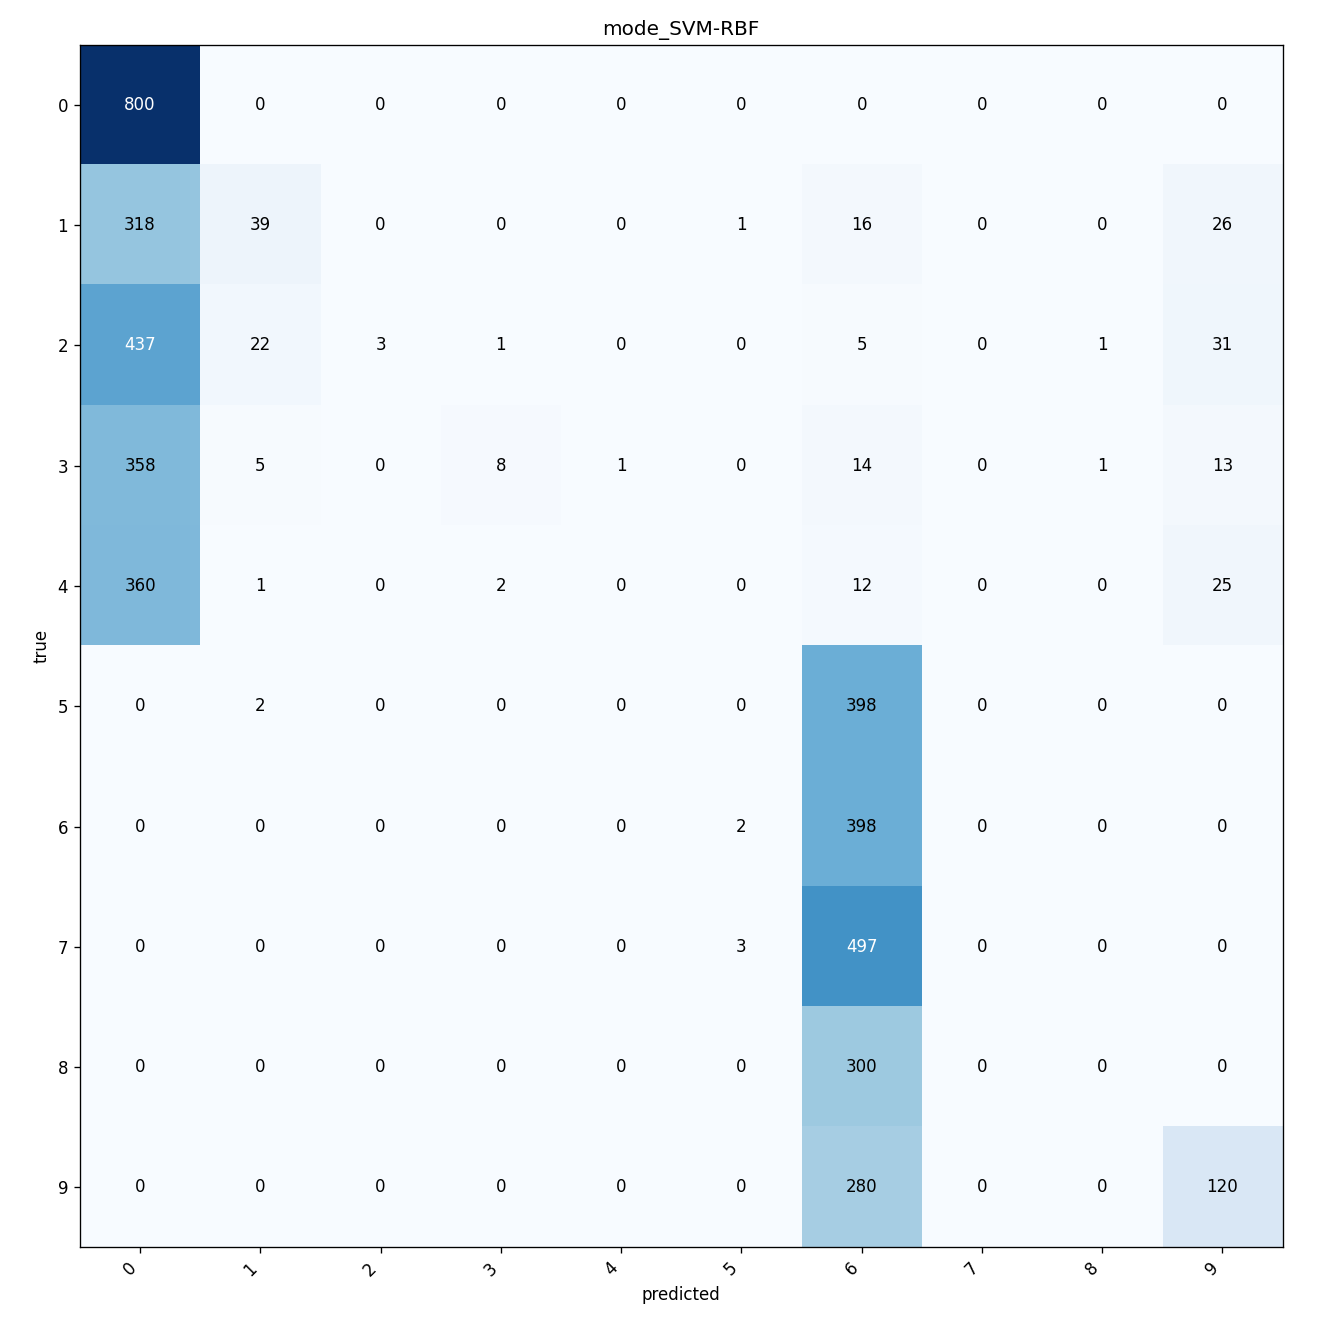
\includegraphics[height=0.40\textheight]{figs/cmmode_SVM-RBF.png}\hfill
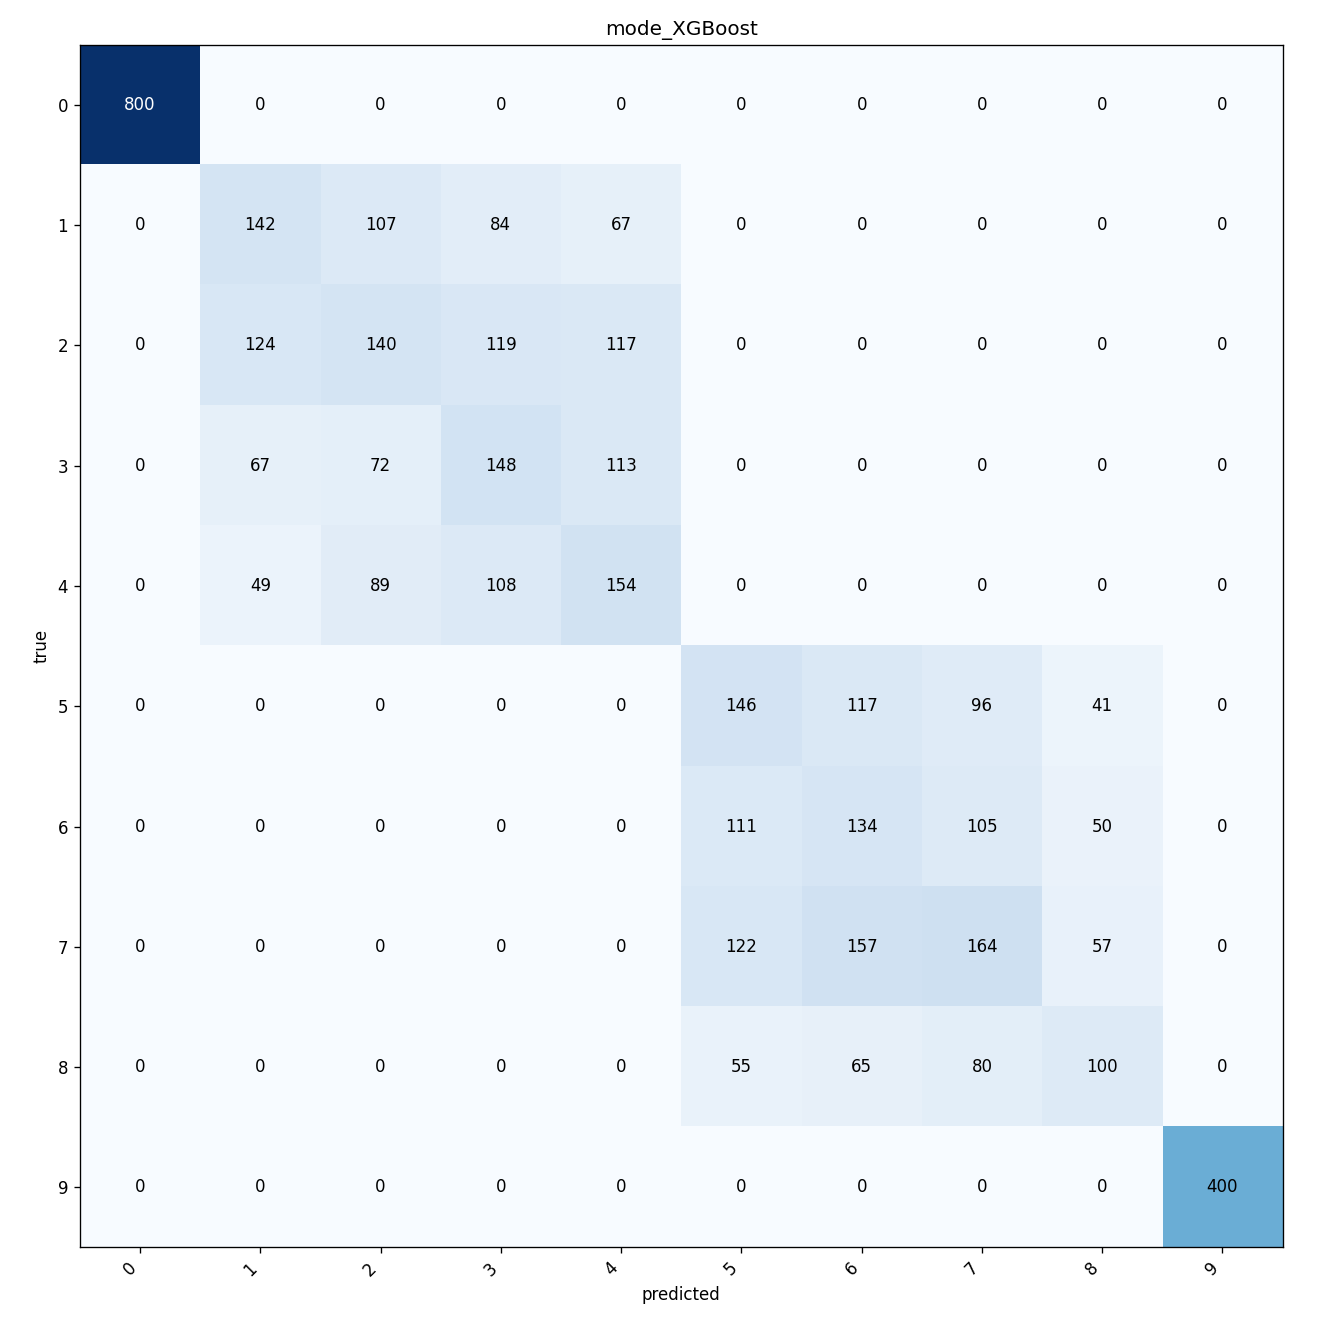
\includegraphics[height=0.40\textheight]{figs/cmmode_XGBoost.png}

\footnotesize Top: Logistic Regression, Random Forest. Bottom: Support Vector
Machine, XGBoost. XGBoost (bottom-right) shows the strongest diagonal, confirming
its lead on the mode task.
\end{frame}

% ============ NOISE ROBUSTNESS ============
\begin{frame}{Robustness Under Noise and Interference}
\begin{columns}[c]
\begin{column}{0.54\textwidth}
\centering
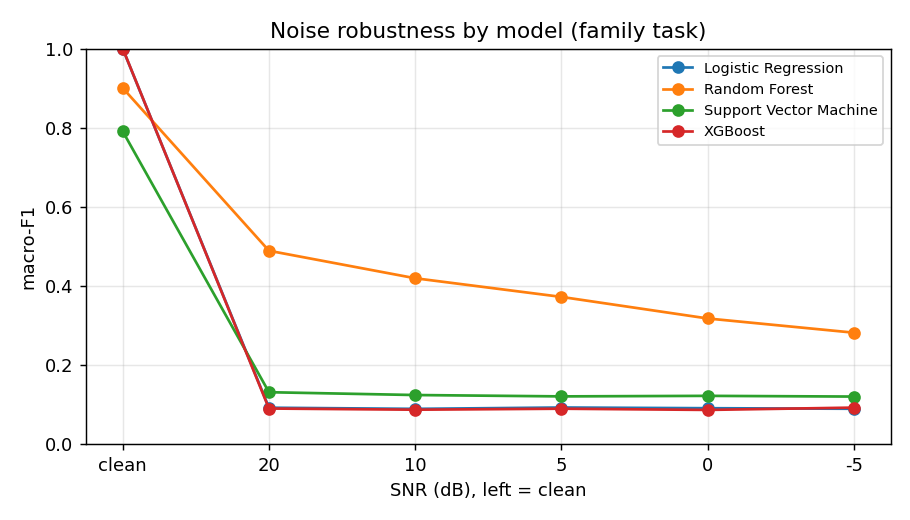
\includegraphics[width=\textwidth]{figs/noise_all.png}
\end{column}
\begin{column}{0.44\textwidth}
\footnotesize
\textbf{Method:} each model is trained on clean data, then evaluated on the
family task as \textbf{Gaussian noise} is added to the test set at decreasing
\textbf{Signal-to-Noise Ratio (SNR)}.
\vspace{0.15cm}

\textbf{Finding:} \textbf{Random Forest} is the most robust, degrading
gracefully. The models with the highest clean scores (XGBoost, Logistic
Regression, Support Vector Machine) collapse to near-chance once any noise is
added.
\vspace{0.15cm}

\textbf{Implication:} high clean accuracy does not imply robustness. A deployed
system would favour Random Forest or require explicit noise handling.
\end{column}
\end{columns}
\end{frame}

% ============ ADVANTAGES + LIMITATIONS ============
\begin{frame}{Advantages and Limitations}
\begin{columns}[t]
\begin{column}{0.49\textwidth}
\textbf{Advantages}
\begin{itemize}\footnotesize
\item \textbf{Passive detection} without line of sight or lighting constraints.
\item \textbf{Interpretable, low-cost} models that train rapidly on standard
hardware.
\item \textbf{Leakage-aware} evaluation yields trustworthy metrics.
\item A single pipeline answers all three classification questions.
\end{itemize}
\end{column}
\begin{column}{0.49\textwidth}
\textbf{Limitations}
\begin{itemize}\footnotesize
\item \textbf{Operating-mode} classification remains difficult (best F1 0.492).
\item Spectral features \textbf{degrade sharply} under heavy noise.
\item Only \textbf{three drone families} are represented in the dataset.
\item Dataset-based study; \textbf{no live hardware} or field deployment.
\end{itemize}
\end{column}
\end{columns}
\end{frame}

% ============ APPLICATIONS + CONCLUSION ============
\begin{frame}{Applications and Conclusion}
\begin{columns}[t]
\begin{column}{0.49\textwidth}
\textbf{Applications}
\begin{itemize}\footnotesize
\item \textbf{Passive surveillance} near airports and restricted zones.
\item Early warning for unauthorised drones at public events.
\item Low-cost monitoring on \textbf{software-defined radios}.
\item Drone-type identification for \textbf{threat assessment}.
\end{itemize}
\end{column}
\begin{column}{0.49\textwidth}
\textbf{Conclusion}
\begin{itemize}\footnotesize
\item Four classical models were compared across three tasks under a
\textbf{leakage-aware} split.
\item Presence and family are reliably classified; \textbf{XGBoost} leads the
hard mode task at 0.492.
\item A \textbf{noise-robustness} test quantified feature sensitivity to
interference.
\item Classical models remain \textbf{competitive with deep learning} on this
dataset.
\end{itemize}
\end{column}
\end{columns}
\end{frame}

% ============ LITERATURE SURVEY ============
\begin{frame}{Literature Survey}
\scriptsize
\begin{tabular}{|p{3.1cm}|p{2.9cm}|p{5.5cm}|}
\hline
\textbf{Reference} & \textbf{Approach} & \textbf{Relevance to the present work} \\
\hline
Al-Sa'd \textit{et al.}, 2019 & Deep Neural Networks &
Established the DroneRF dataset and the three-task structure adopted here. \\
\hline
Al-Emadi \textit{et al.}, 2020 & XGBoost, three tasks &
Closest prior study; corroborates XGBoost's strength and the difficulty of the
mode task. \\
\hline
Ezuma \textit{et al.}, 2020 & Machine learning under interference &
Motivates the noise-robustness analysis in the shared 2.4~GHz band. \\
\hline
Medaiyese \textit{et al.}, 2022 & Wavelet-transform features &
Principal alternative to the Fast Fourier Transform features used here. \\
\hline
LUMEN, 2026 & Power Spectral Density features &
Validates the power-spectral feature choice on constrained hardware. \\
\hline
Sensors, 2024 & RF detector robustness study &
Establishes Signal-to-Noise-Ratio degradation testing as standard practice. \\
\hline
\end{tabular}
\vspace{0.2cm}

\footnotesize\textbf{Research gap:} prior studies are largely deep-learning-based
or omit an explicit leakage check. This work compares four interpretable
classical models across all three tasks under a recording-grouped split.
\end{frame}

% ============ REFERENCES ============
\begin{frame}{References}
\scriptsize
\begin{enumerate}
\item M. F. Al-Sa'd \textit{et al.}, ``RF-based drone detection and
identification using deep learning approaches,'' \textit{Future Generation
Computer Systems}, vol. 100, 2019.
\item S. Al-Emadi, F. Al-Senaid, ``Drone detection using machine learning,''
\textit{Proceedings of the IEEE International Conference on Informatics, IoT and
Enabling Technologies}, 2020.
\item M. Ezuma \textit{et al.}, ``Detection and classification of UAVs in the
presence of Wi-Fi and Bluetooth interference,'' \textit{IEEE Open Journal of the
Communications Society}, vol. 1, 2020.
\item O. O. Medaiyese \textit{et al.}, ``Wavelet transform analytics for
RF-based UAV detection,'' \textit{Pervasive and Mobile Computing}, vol. 82, 2022.
\item ``LUMEN: a lightweight UAV network for Power Spectral Density-based RF
fingerprinting,'' \textit{Sensors}, vol. 26(10), 2026.
\item ``Robustness of deep-learning-based RF UAV detectors,'' \textit{Sensors},
vol. 24(22), 2024.
\item M. S. Allahham \textit{et al.}, ``DroneRF dataset,'' \textit{Data in
Brief}, vol. 26, 2019.
\end{enumerate}
\end{frame}

\end{document}
